\section{Ausblick}\label{sec:outlook}
In diesem Abschnitt werden mögliche Erweiterungen für den Begriffsverband vorgestellt.
Im Vergleich zum vorherigen \autoref{sec:discussion} werden hier Ansätze vorgestellt, welche bereits zu einem gewissen Teil untersucht wurden.
Alle hier genannten Ansätze sind jedoch nicht umgesetzt oder explizit teil dieser Arbeit.
Stattdessen werden diese Ansätze als mögliche Erweiterungen vorgestellt, welche in zukünftigen Arbeiten oder Iterationen des Prototyps umgesetzt werden können.
Dabei ist zu beachten, dass diese Ansätze nicht vollständig untersucht wurden und daher nur als Ideen zu verstehen sind.
Es gilt diese empirisch zu untersuchen und zu evaluieren, ob diese Ansätze tatsächlich einen Mehrwert für die Nutzenden bieten. \\

\begin{figure}[!ht]
    \centering
    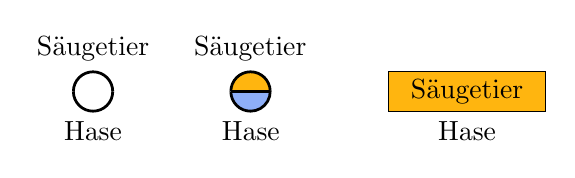
\begin{tikzpicture}
        \definecolor{nodeyellow}{HTML}{FFB50F}
        \definecolor{nodeblue}{HTML}{8EAFF8}

        \draw[line width=1pt] (0,0) arc (180:0:0.25) node[midway,above] {Säugetier};
        \draw[line width=1pt] (0,0) arc (-180:0:0.25) node[midway,below] {Hase}; 

        \draw[line width=1pt, fill=nodeyellow] (2,0) arc (180:2:0.25) node[midway,above] {Säugetier};
        \draw[line width=1pt, fill=nodeblue] (2,0) arc (-180:2:0.25) node[midway,below] {Hase}; 
        \draw[line width=1pt] (2,0) -- (2.5,0);

        \draw[fill=nodeyellow] (4,-0.25) rectangle (6,0.25) node[midway] {Säugetier};
        \node at (5,-0.5) {Hase};
    \end{tikzpicture}
    \caption{\label{fig:node-types}Arten der Knotenrepräsentation}
\end{figure}

% Knotentypen
In \autoref{fig:node-types} sind drei verschiedene Möglichkeiten dargestellt Knoten in einem Begriffsverband zu repräsentieren.
Die linke Darstellung repräsentiert einen Knoten, welcher in dieser Form häufig in der Literatur zu finden ist.
Mittig ist die Darstellung, welche in der Vorstudie und in dieser Arbeit verwendet wurde.
Durch die Verwendung von Farben wird die Zuordnung in Merkmal und Gegenstand visuell unterstützt.
Rechts ist eine weitere Möglichkeit, bei der ein Merkmal in einem Rechteck dargestellt wird und die zugehörigen Gegenstände unterhalb des Rechtecks aufgelistet werden.
In dieser Arbeit wurde zunächst die mittlere Darstellung verwendet, um eine bessere Vergleichbarkeit mit der Vorstudie zu gewährleisten.
Durch das Rechteck hingegen könnte die Zuordnung von Merkmal und Gegenstand deutlicher werden.
In zukünftigen Arbeiten sollte daher untersucht werden, welche Darstellung für die Nutzenden besser geeignet ist.
Eine Interkation, welche zuvor mit dem unteren Halbkreis durchgeführt wurde, würde beim Rechteck entfallen, da das Rechteck keine zwei Interaktionsflächen bietet.
Diese Interaktion ist jedoch nicht zwingend notwendig, da nur die Artikel des angeklickten Knotens angezeigt werden.
Durch die Interaktion mit einem Merkmal wird jedoch der Umfang eines Begriffs aufgeführt, welcher die Artikel des angeklickten Knotens enthält.\\

% Statistik
Durch die Kategorisierung von Artikeln in die \ac{EC} werden neue Möglichkeiten geschaffen, um die Artikel weiter zu analysieren.
Dies schafft zusätzlich weitere Möglichkeiten die Bevölkerung zu informieren.
Es könnten beispielsweise Statistiken erstellt werden, welche Aufschluss über die Anzahl der Artikel geben, welche in die einzelnen Kategorien fallen.
In den Interviews ist aufgefallen, dass die Artikel aus dem Datensatz sich größtenteils positiv bezüglich der Welten der \ac{EC} rechtfertigen.
Wird dies verknüpft mit der Quelle der Artikel, könnte eine Statistik Aufschluss über die Rechtfertigungen eines Mediums geben.
Ebenfalls wäre es möglich, dass die Artikel journalistisch tätiger Personen analysiert werden.
Durch eine sinnvoll gewählte Repräsentation dieser Daten wäre es möglich auf einem Blick zu erkennen, ob eine Redaktion ein breites Spektrum an Welten abdeckt oder sich auf bestimmte Welten und Rechtfertigungen spezialisiert hat.
Für Nutzende könnte dies ein Indikator sein, sich selbst bewusst zu werden, ob das favorisierte Nachrichtenmagazin eine bestimmte Weltsicht vertritt. \\

% Cluster 
Da es journalistischen Standards entspricht, dass Artikel durch ausreichend Quellen belegt werden, entstand die Idee diese Quellen verpflichtend angeben zu lassen.
Dies würde eine weitere Möglichkeit schaffen Nutzende zu informieren und ihnen die Möglichkeit zu geben, sich selbst ein Bild über die Quellen von Artikeln zu machen.
Eine sinnvolle Darstellung dieser Quellen könnte durch die Verwendung von Clustern erreicht werden.
Dabei werden Artikel mit gleichen Quellen in einem Cluster zusammengefasst.
Dieser Ansatz kann verwendet werden, um Zusammenhänge oder Abhängigkeiten zwischen Artikeln zu erkennen.
Nutzende könnten auf diese Weise schnell erkennen, dass mehrere Artikel die gleiche Quelle verwenden.
Durch die Verwendung von Clustern könnten Nutzende erkennen, dass sie sich in einer Filterblase befinden, da sie nur Artikel aus einem Cluster lesen.
